
%(BEGIN_QUESTION)
% Copyright 2011, Tony R. Kuphaldt, released under the Creative Commons Attribution License (v 1.0)
% This means you may do almost anything with this work of mine, so long as you give me proper credit

The following Ethernet network has a problem.  Someone trying to access the Internet from personal computer \#4 cannot do so, and has called you to troubleshoot the problem:

$$\includegraphics[width=15.5cm]{i04461x01.eps}$$

Your first diagnostic test is to ``ping'' computer \#4 from computer \#5, and you find that this test is successful.  Your next test is to check Internet connectivity at computer \#5 by ``pinging'' {\tt http://www.google.com}, and you find that test is successful as well. 

Identify the likelihood of each specified fault for this network.  Consider each fault one at a time (i.e. no coincidental faults), determining whether or not each fault could independently account for {\it all} measurements and symptoms in this network.

% No blank lines allowed between lines of an \halign structure!
% I use comments (%) instead, so that TeX doesn't choke.

$$\vbox{\offinterlineskip
\halign{\strut
\vrule \quad\hfil # \ \hfil & 
\vrule \quad\hfil # \ \hfil & 
\vrule \quad\hfil # \ \hfil \vrule \cr
\noalign{\hrule}
%
% First row
{\bf Fault} & {\bf Possible} & {\bf Impossible} \cr
%
\noalign{\hrule}
%
% Another row
Hub A failed &  &  \cr
%
\noalign{\hrule}
%
% Another row
Hub B failed &  &  \cr
%
\noalign{\hrule}
%
% Another row
Router failed &  &  \cr
%
\noalign{\hrule}
%
% Another row
Internet service provider failed &  &  \cr
%
\noalign{\hrule}
%
% Another row
Cable failed between computer \#4 and Hub B &  &  \cr
%
\noalign{\hrule}
%
% Another row
Cable failed between Hub A and Router &  &  \cr
%
\noalign{\hrule}
%
% Another row
Cable failed between Hub B and Router &  &  \cr
%
\noalign{\hrule}
%
% Another row
Security settings (e.g. firewall) in computer \#4 &  &  \cr
%
\noalign{\hrule}
} % End of \halign 
}$$ % End of \vbox

Finally, identify the {\it next} diagnostic test or measurement you would make on this system.  Explain how the result(s) of this next test or measurement help further identify the location and/or nature of the fault.

\underbar{file i04461}
%(END_QUESTION)





%(BEGIN_ANSWER)

\noindent
{\bf Partial answer:}

% No blank lines allowed between lines of an \halign structure!
% I use comments (%) instead, so that TeX doesn't choke.

$$\vbox{\offinterlineskip
\halign{\strut
\vrule \quad\hfil # \ \hfil & 
\vrule \quad\hfil # \ \hfil & 
\vrule \quad\hfil # \ \hfil \vrule \cr
\noalign{\hrule}
%
% First row
{\bf Fault} & {\bf Possible} & {\bf Impossible} \cr
%
\noalign{\hrule}
%
% Another row
Hub A failed &  &  \cr
%
\noalign{\hrule}
%
% Another row
Hub B failed &  &  \cr
%
\noalign{\hrule}
%
% Another row
Router failed &  & $\surd$ \cr
%
\noalign{\hrule}
%
% Another row
Internet service provider failed &  & $\surd$ \cr
%
\noalign{\hrule}
%
% Another row
Cable failed between computer \#4 and Hub B &  & \cr
%
\noalign{\hrule}
%
% Another row
Cable failed between Hub A and Router &  & $\surd$ \cr
%
\noalign{\hrule}
%
% Another row
Cable failed between Hub B and Router &  &  \cr
%
\noalign{\hrule}
%
% Another row
Security settings (e.g. firewall) in computer \#4 &  &  \cr
%
\noalign{\hrule}
} % End of \halign 
}$$ % End of \vbox

%(END_ANSWER)





%(BEGIN_NOTES)

% No blank lines allowed between lines of an \halign structure!
% I use comments (%) instead, so that TeX doesn't choke.

$$\vbox{\offinterlineskip
\halign{\strut
\vrule \quad\hfil # \ \hfil & 
\vrule \quad\hfil # \ \hfil & 
\vrule \quad\hfil # \ \hfil \vrule \cr
\noalign{\hrule}
%
% First row
{\bf Fault} & {\bf Possible} & {\bf Impossible} \cr
%
\noalign{\hrule}
%
% Another row
Hub A failed &  & $\surd$ \cr
%
\noalign{\hrule}
%
% Another row
Hub B failed &  & $\surd$ \cr
%
\noalign{\hrule}
%
% Another row
Router failed &  & $\surd$ \cr
%
\noalign{\hrule}
%
% Another row
Internet service provider failed &  & $\surd$ \cr
%
\noalign{\hrule}
%
% Another row
Cable failed between computer \#4 and Hub B &  & $\surd$ \cr
%
\noalign{\hrule}
%
% Another row
Cable failed between Hub A and Router &  & $\surd$ \cr
%
\noalign{\hrule}
%
% Another row
Cable failed between Hub B and Router &  & $\surd$ \cr
%
\noalign{\hrule}
%
% Another row
Security settings (e.g. firewall) in computer \#4 & $\surd$ &  \cr
%
\noalign{\hrule}
} % End of \halign 
}$$ % End of \vbox


\vskip 10pt

5 can ping 4, which tells us all the cabling between those two PCs are fine, as is the hub between them.  5 can also ping Google, which indicates we have a connection with the outside world, and that the right hub is completely fine, and that the router is working (at least on that side of the network).  The problem, then, appears to be within 4.

\vskip 10pt

Pinging {\tt http://www.google.com} from computer \#4 is a good diagnostic test, to see if DNS (Domain Name Services) is running in that computer.








\vskip 20pt \vbox{\hrule \hbox{\strut \vrule{} {\bf Virtual Troubleshooting} \vrule} \hrule}

This question is a good candidate for a ``Virtual Troubleshooting'' exercise.  Presenting the diagram to students, you first imagine in your own mind a particular fault in the system.  Then, you present one or more symptoms of that fault (something noticeable by an operator or other user of the system).  Students then propose various diagnostic tests to perform on this system to identify the nature and location of the fault, as though they were technicians trying to troubleshoot the problem.  Your job is to tell them what the result(s) would be for each of the proposed diagnostic tests, documenting those results where all the students can see.

During and after the exercise, it is good to ask students follow-up questions such as:

\begin{itemize}
\item{} What does the result of the last diagnostic test tell you about the fault?
\item{} Suppose the results of the last diagnostic test were different.  What then would that result tell you about the fault?
\item{} Is the last diagnostic test the best one we could do?
\item{} What would be the ideal order of tests, to diagnose the problem in as few steps as possible?
\end{itemize}

%INDEX% Networking, Ethernet: troubleshooting using "ping"

%(END_NOTES)

